\documentclass[border=5pt]{standalone}
\usepackage{pgfplots}
\pgfplotsset{compat=1.18}
\begin{document}
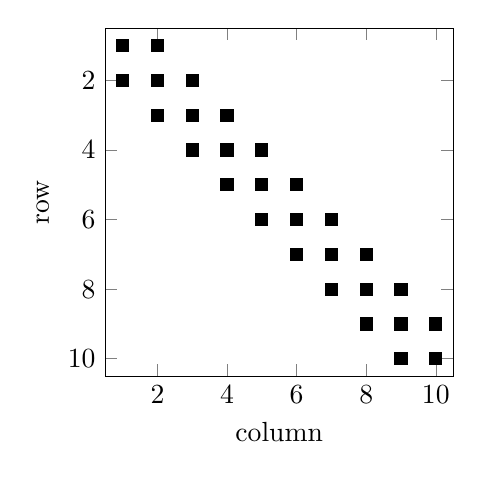
\begin{tikzpicture}
\begin{axis}[
    width=6cm, height=6cm, y dir=reverse, axis equal image,
    xmin=0.5, xmax=10.5, ymin=0.5, ymax=10.5,
    xlabel={column}, ylabel={row},
]
% 1D Laplacian: tridiagonal pattern
\addplot[only marks, mark=square*, mark size=2.2pt,
    variable=\i, samples at={1,...,10}] ({\i},{\i});
\addplot[only marks, mark=square*, mark size=2.2pt,
    variable=\i, samples at={1,...,9}] ({\i+1},{\i});
\addplot[only marks, mark=square*, mark size=2.2pt,
    variable=\i, samples at={1,...,9}] ({\i},{\i+1});
\end{axis}
\end{tikzpicture}
\end{document}
